\section{Theorie}
\label{sec:Theorie}
  Das Herstellen einer Besetzungsinversion meint die induzierte Abkehr von der thermischen Besetzungswahrscheinlichkeit der Energieniveaus eines Atoms.
  Um dies zu verstehen, ist es zunächst nötig, die elektronische Struktur des hier untersuchten Elements Rubidium zu erläutern.

  \subsection{Beschreibung der Energieniveaus in Rubidium}
  \label{subsec:energieniveaus}
  Bei Rubidium handelt es sich um ein Erdalkalimetall, das nur über ein ungepaartes Elektron in der fünften Schale verfügt, sodass nur dieses zu den Quantenzahlen der Elektronenhülle beiträgt.
  Ohne Betrachtung von Korrekturen befindet es sich als Spin-1/2-Teilchen in dem Zustand mit $n=5$, $l=0$ und $m_l=0$, wobei $n$ die Hauptquantenzahl, $l$ die Neben- oder auch Drehimpulsquantenzahl und $m_l$ die zu ihr gehörige magnetische Quantenzahl bezeichnet. In niedrigster Ordnung verfügt das Niveau mit $l=1$ und $m_l=0,\pm1$ über die gleiche Energie wie der besetzte Zustand, sie sind entartet.

  Die Berücksichtigung der Spin-Bahn-Kopplung zeigt allerdings, dass dies nicht der Fall ist: Der Bahndrehimpuls $\vec{L}$ und der Spin $\vec{S}$ des Elektrons addieren sich vektoriell zu einem Gesamtdrehimpuls $\vec{J}=\vec{L}+\vec{S}$, sodass dieser eine Erhaltungsgröße darstellt. Die Quantenzahlen $j$ und $m_j$ definieren nun statt $l$ und $m_l$ einen gegebeben Zustand, wobei $j$ von $\lvert L - S \rvert$ bis $\lvert L + S \rvert$ reicht. Zustände mit verschiedenem $j$ sind in dieser Feinstruktur nicht mehr energetisch entartet, während Zustände mit gleichem $j$ und verschiedenem $m_j$ ohne äußeres Magnetfeld energetisch entartet bleiben.
  Die Feinstruktur ist als gröbste Aufspaltung links in Abbildung \ref{fig:energieniveaus} zu sehen.

  \begin{figure}
    \centering
    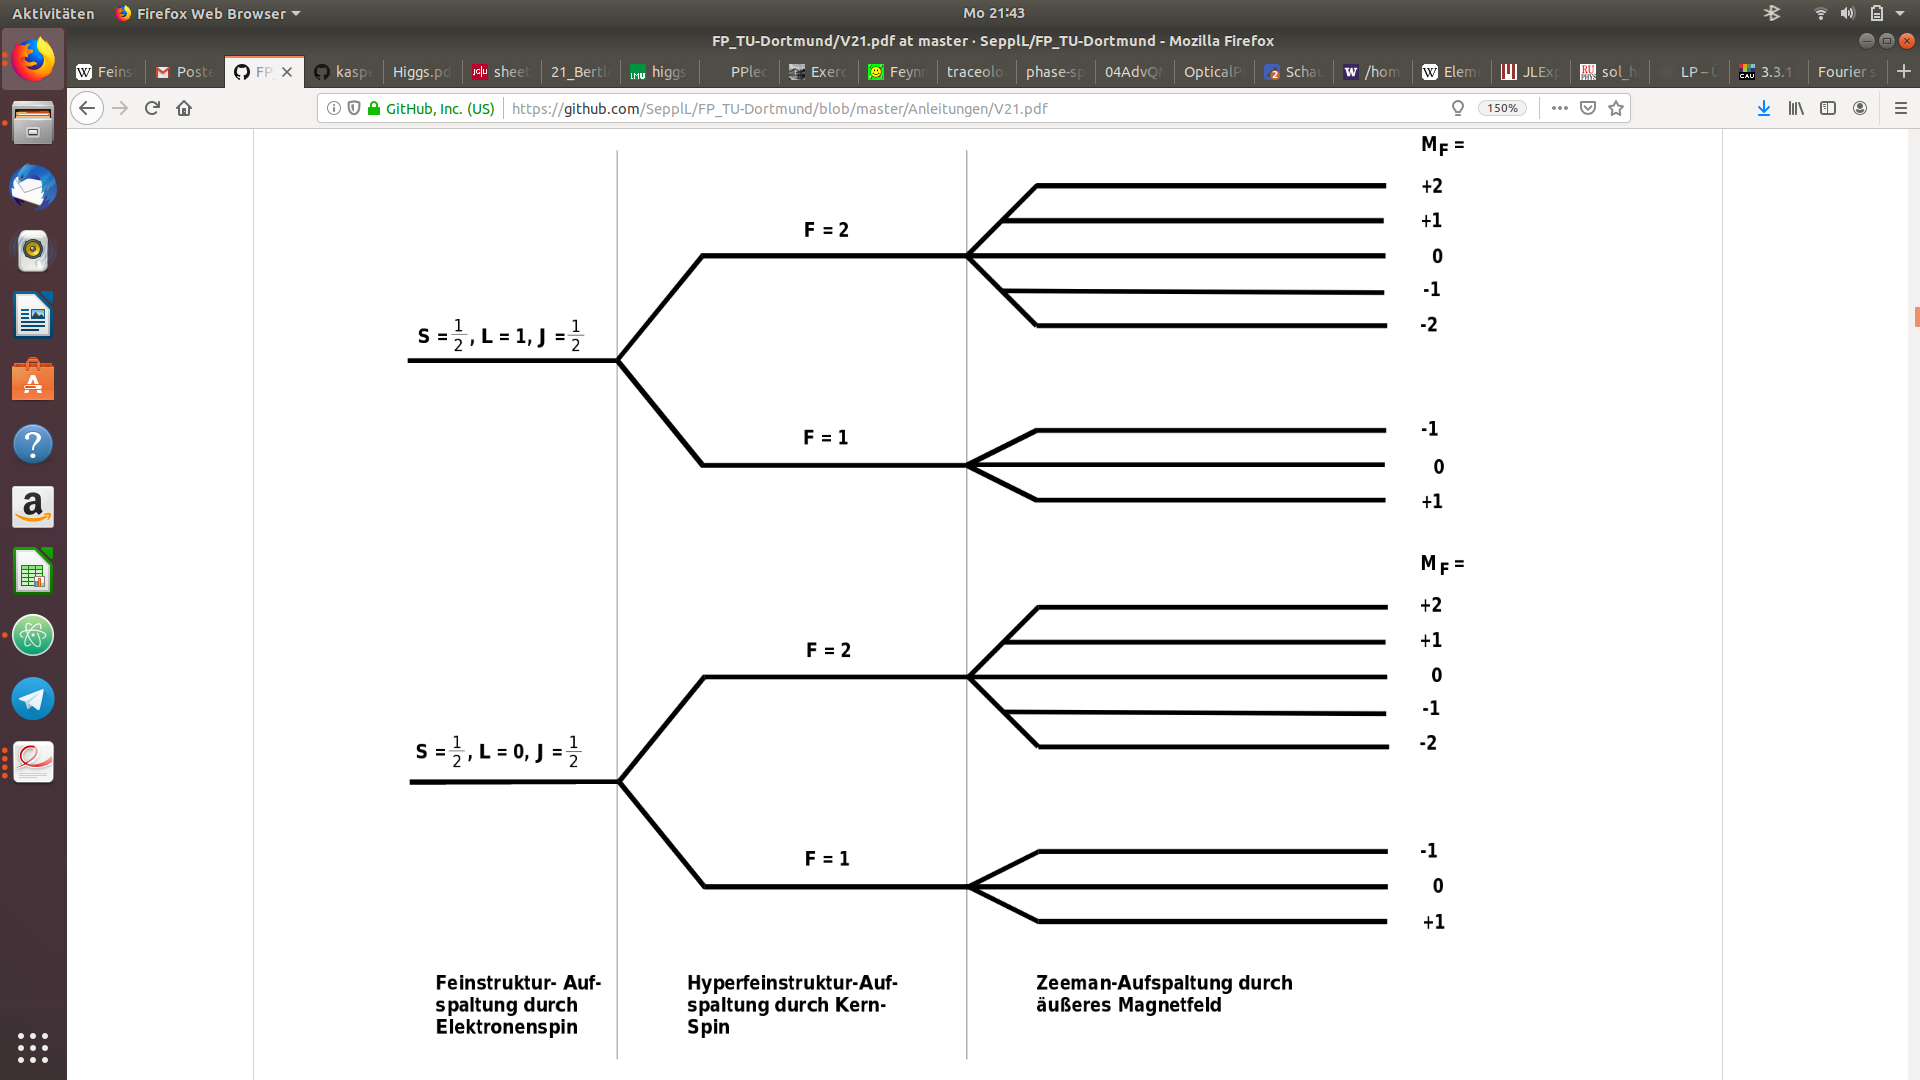
\includegraphics[width=\textwidth]{pictures/energieniveaus.png}
    \caption{Energieniveaus in \ce{^{87}Rb} mit $I=3/2$ (nicht maßstäblich) \cite{stehendeWelle}.}
    \label{fig:energieniveaus}
  \end{figure}

  Die Feinstrukturniveaus spalten in weiterer Korrektur auf, wenn die Spin-Spin-Kopplung des Kernspins an den Gesamtdrehimpuls der Elektronenhüllen berücksichtigt wird. Dazu wird der Gesamtdrehimpuls $\vec{F}$ des Atoms wieder durch Vektoraddition gebildet: $\vec{F} = \vec{J} + \vec{I}$. Zu diesem gehört die Quantenzahl $F$, die Werte von $\lvert J - I \rvert$ bis $\lvert J + I \rvert$ annimmt, mit der magnetischen Quantenzahl $m_F$. Im Beispiel in Abbildung \ref{fig:energieniveaus} werden die Feinstrukturniveaus dementsprechend jeweils in zwei Niveaus aufgespalten, wobei wieder Zustände mit gleichem $F$ und verschiedenem $m_F$ ohne äußeres Magnetfeld energetisch entartet bleiben.

  Die Aufhebung der Entartung dieser Zustände durch ein Magnetfeld geschieht durch den sogenannten Zeeman-Effekt. Dieser spaltet einen $F$-Zustand wiederum in $2F$+1-Zustände auf. Die Energiedifferenz zweier benachbarter Zeeman-Niveaus beträgt
  \begin{equation}
    \Delta E_Z = g_F \mu_B B
    \label{eqn:zeemanDifferenz}
  \end{equation}
  und ist somit proportional zur magnetischen Flussdichte $B$. Der Faktor $\mu_B = \frac{e \hbar}{2m_e}$ ist das Bohrsche Magneton, das kleinstmögliche magnetische Moment, das ein Elektron tragen kann. Der Landé-Faktor des Gesamtdrehimpulses des Atoms $g_F$ ergibt sich aus Kopplungsdiagrammen der beteiligten Drehimpulse näherungsweise zu
  \begin{equation}
    g_F = g_J \frac{F(F+1)+J(J+1)-I(I+1)}{2F(F+1)}\,,
    \label{eqn:g_F_Theorie}
  \end{equation}
  wobei der Landé-Faktor des Gesamtdrehimpulses des Elektrons
  \begin{equation}
    g_J = \frac{3,0023J(J+1)+1,0023(S(S+1)-L(L+1))}{2J(J+1)}
    \label{eqn:g_J_Theorie}
  \end{equation}
  beträgt.

  \section{Prinzip des optischen Pumpens und der Hochfrequenzspektroskopie}
  \label{subsec:prinzipOptischesPumpen}

  Es ist üblich, die Feinstrukturniveaus als Termsymbole ${}^{2S+1}L_J$ mit der Multiplizität $2S+1$ und dem Kennbuchstaben $L$ für den elektronischen Drehimpuls zu schreiben, wobei für $L=0$ ein S und für $L=1$ ein P geschrieben wird.

  Für das optische Pumpen an Rubidium ist die Aufspaltung der Hyperfeinstrukturniveaus durch den Zeeman-Effekt nötig. Ohne äußere, zeitabhängige Störung folgt die Besetzung dann näherungsweise einer thermischen Boltzmann-Verteilung, sodass die Elektronen größtenteils im Grundzustand mit niedrigstem $m_F$ angereichert sind.

  Es wird nun rechtszirkular polarisiertes Licht der Frequenz des $D_1$-Übergangs eingestrahlt, dessen Energie dem Übergang von ${}^{2}P_{1/2}$ nach ${}^{2}S_{1/2}$ entspricht. Übergänge, die durch Absorption dieser Photonen entstehen, gehorchen der Auswahlregel $m_F=+1$, während die spontane Emission keine bestimmten Übergänge bevorzugt. Es gelingt also, durch dieses Prinzip den niedrigsten Zustand nahezu leer zu pumpen und den S-Zustand mit $F=2$, $m_F=2$ anzureichern und eine Besetzungsinversion herbeizuführen. Eine schematische Darstellung der Übergänge findet sich in Abbildung \ref{fig:pumpschema}

  \begin{figure}
    \centering
    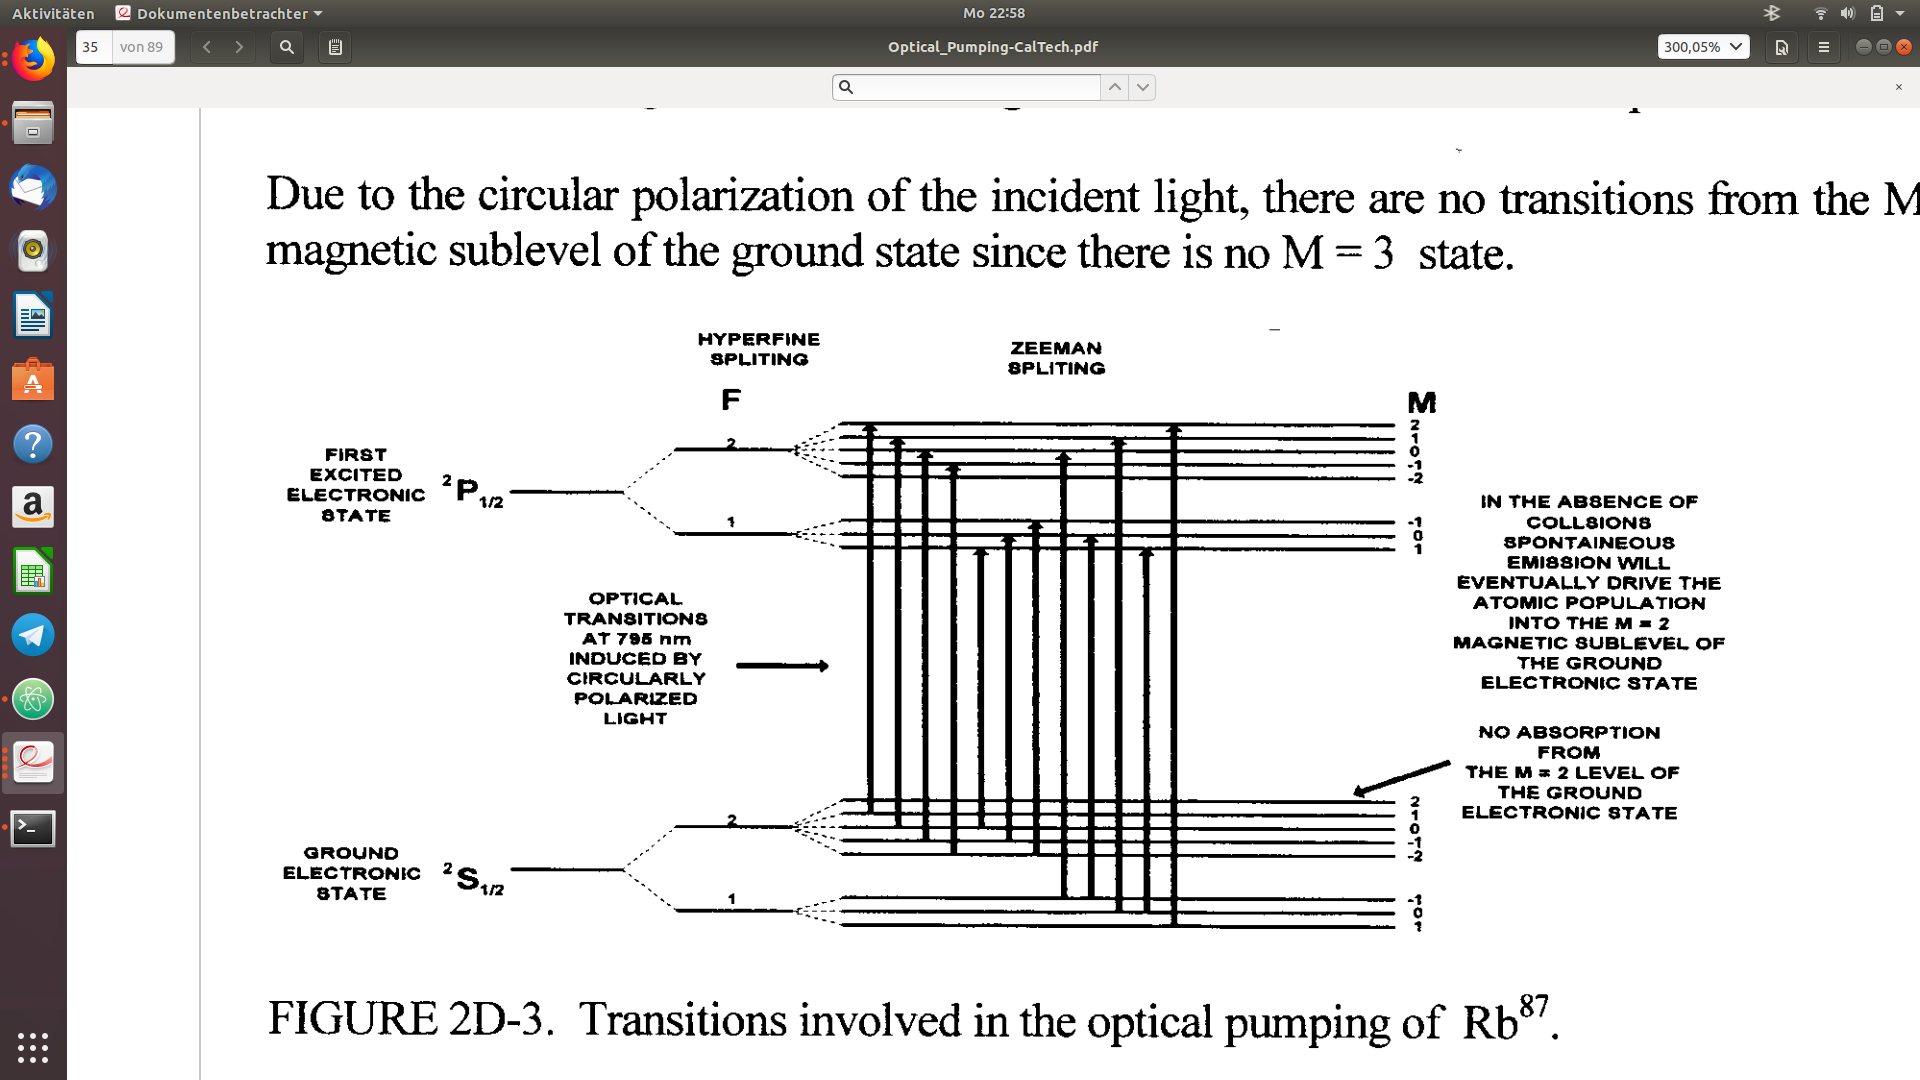
\includegraphics[width=\textwidth]{pictures/pumpschema.png}
    \caption{insert description \cite{stehendeWelle}.}
    \label{fig:pumpschema}
  \end{figure}

  Ein geeignetes Maß für die Besetzungsinversion stellt die Transparenz der Dampfzelle gegenüber dem einstrahlenden $D_1$-Licht dar. Diese wird mit einer ansteigenden Exponentialfunktion parametrisiert, welche sich bei vollständiger Inversion sättigt, da das Licht dann aufgrund der Auswahlregel keinen Übergang anregen kann.

  \cite{insert Bild?}

  \cite{FRAGE: EINFACH IMMER GROßBUCHSTABEN FÜR DIE QUANTENZAHLEN, SO WIE IN DER ALTEN ANLEITUNG?}

  Obwohl die Zeeman-Aufspaltung das Phänomen des optischen Pumpens erst möglich macht, wird Letzteres oft als spektroskopisches Verfahren eingesetzt, um die aufgespaltenen Energieniveaus mit hoher Genauigkeit zu vermessen. Dieses Messverfahren bedient sich eines zweiten, hochfrequenten magnetischen Feldes (RF-Feld), welches stimulierte Emission aus dem angereicherten Niveau heraus anregt. Für die dafür benötigte Flussdichte $B_m$ gilt die Beziehung
  \begin{equation}
    h f = g_F \mu_B B_m \Delta M_F \implies B_m = \frac{4 \pi m_e}{e g_F} f\,,
    \label{eqn:B_M_Theorie}
  \end{equation}
  sodass ein linearer Zusammenhang zu der Frequenz des Feldes besteht.
  Da mit der stimulierten Emission eine Entleerung des zuvor angereicherten Niveaus verbunden wird, wird das Erreichen der Feldstärke $B_m$ mit einer deutlichen Abnahme der Transparenz des Gases verbunden sein, weil der konkurrierende Prozess der Besetzungsinversion durch optisches Pumpen wieder aufnehmen kann. Grafisch ist dies in Abbildung \ref{fig:transparenz} dargestellt.

  \begin{figure}
    \centering
    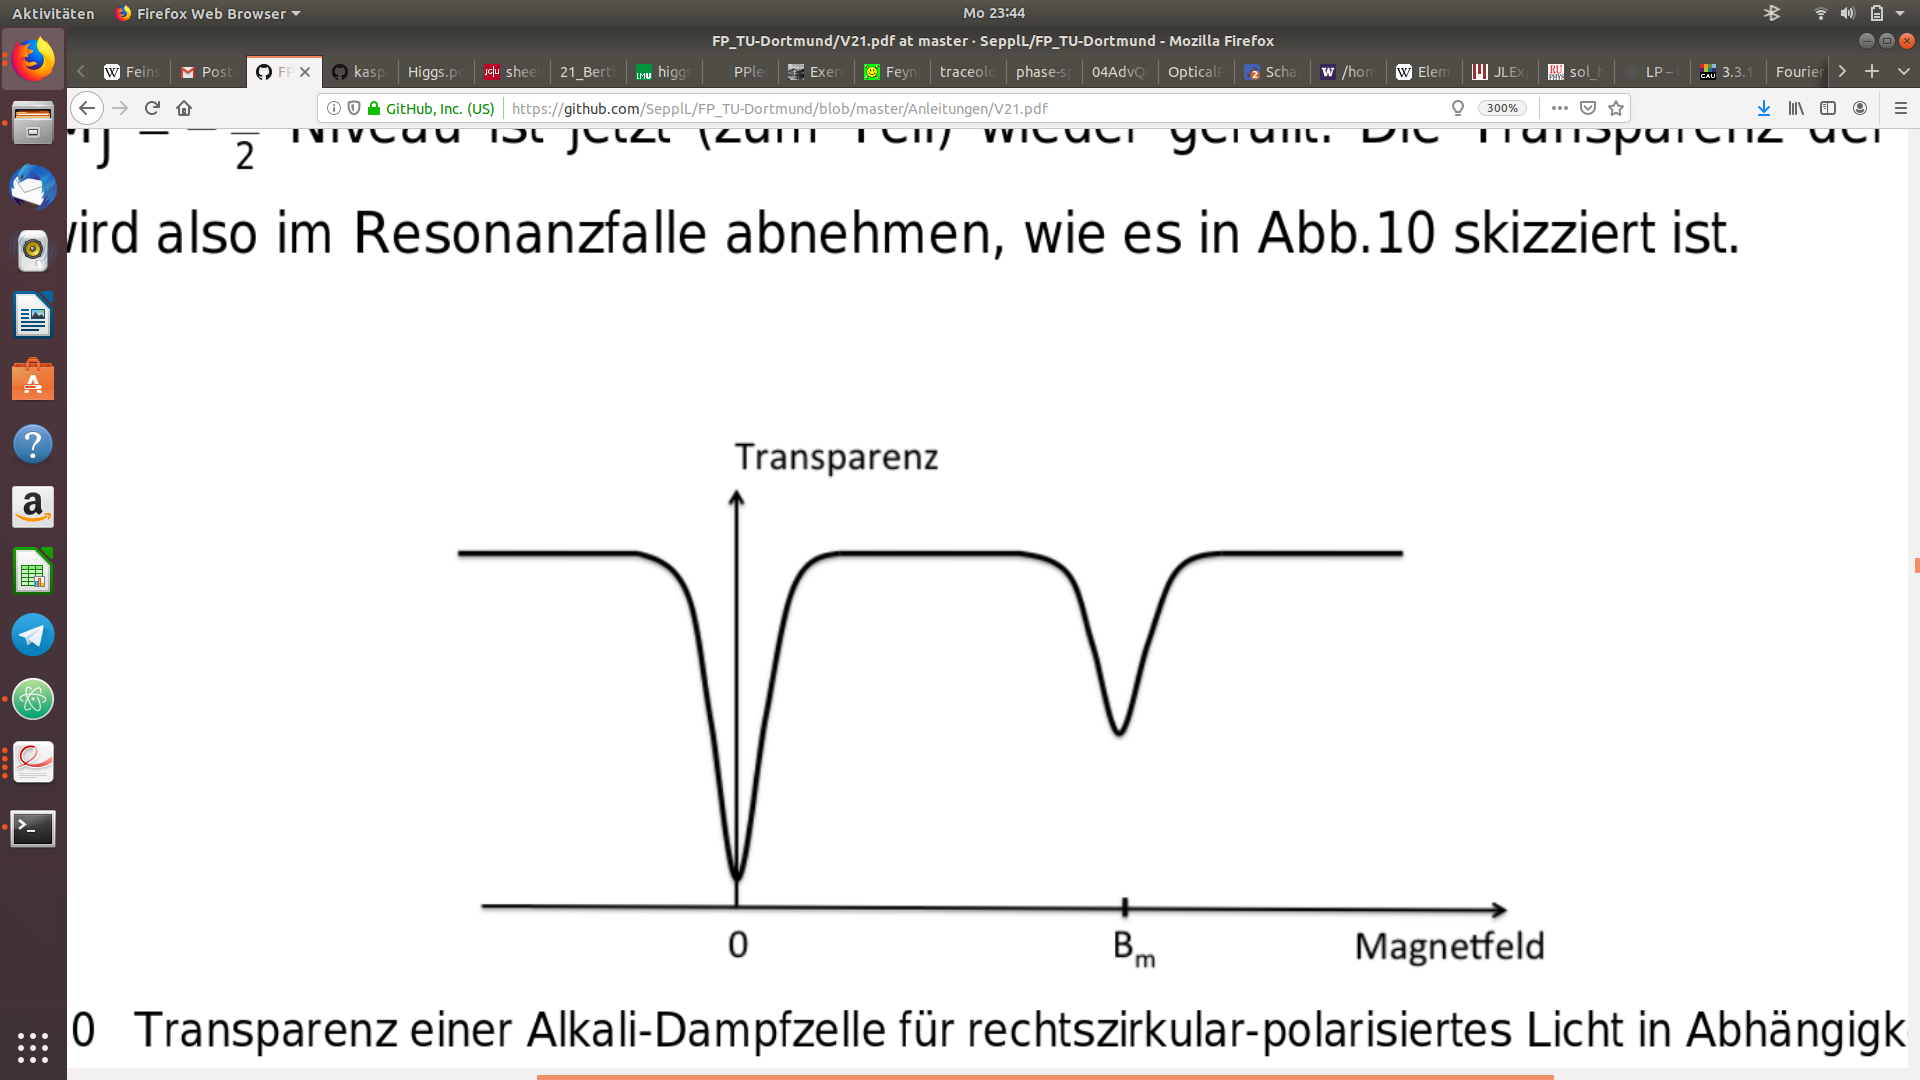
\includegraphics[width=\textwidth]{pictures/transparenz.png}
    \caption{insert description \cite{stehendeWelle}.}
    \label{fig:transparenz}
  \end{figure}

  Um 0 herum sinkt die Transparenz deutlich ab, dort kann keine Besetzungsinversion hergestellt werden. Dies liegt daran, dass dies in einem Zweiniveausystem nicht möglich ist, da die Prozesse der Absorption und der stimulierten Emission miteinander konkurrieren, wobei die zusätzliche spontane Emission die Besetzung des Grundzustandes noch weiter bevorzugt. Experimentell wird dies ausgenutzt, um den Einfluss des Erdmagnetfelds zu minimieren.

  \subsection{Abschätzung des quadratischen Zeeman-Effekts}
  \label{subsec:quadratischerZeeman}

  \subsection{Transiente Effekte}
  \label{subsec:transient}
